\documentclass[tikz,border=2pt]{standalone}
\usepackage{amsmath,amssymb}
\usepackage{tikz}

\begin{document}
% Disconnected: E splits into two non-empty parts kept apart by disjoint open sets U and V.
% Connected: no such split exists (one piece).
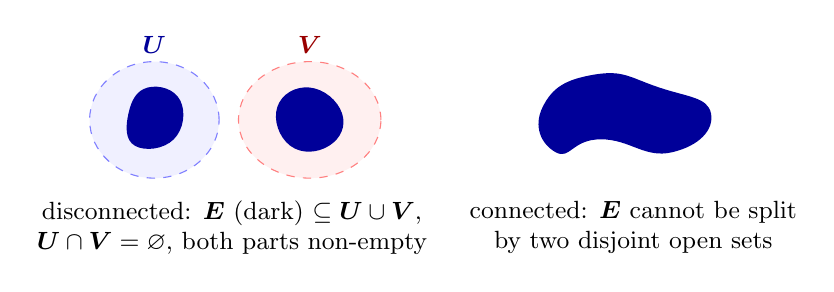
\begin{tikzpicture}[scale=0.822,   every node/.style={font=\small}]
	\draw[blue!50, dashed, fill=blue!6] (-1.1,0) ellipse (1.0 and 0.9);
	\draw[red!50, dashed, fill=red!6] (1.3,0) ellipse (1.1 and 0.9);
	\fill[blue!60!black] plot[smooth cycle, tension=0.8] coordinates {(-1.5,0.1) (-1.2,0.5) (-0.7,0.3) (-0.8,-0.3) (-1.4,-0.4)};
	\fill[blue!60!black] plot[smooth cycle, tension=0.8] coordinates {(0.8,0.2) (1.3,0.5) (1.8,0.1) (1.6,-0.4) (1.0,-0.4)};
	\node[blue!60!black] at (-1.1,1.15) {$\boldsymbol{U}$};
	\node[red!60!black] at (1.3,1.15) {$\boldsymbol{V}$};
	\node[anchor=north, align=center] at (0.1,-1.1) {disconnected: $\boldsymbol{E}$ (dark) $\subseteq\boldsymbol{U}\cup\boldsymbol{V}$,\\ $\boldsymbol{U}\cap\boldsymbol{V}=\varnothing$, both parts non-empty};
	\begin{scope}[xshift=6.3cm]
		\fill[blue!60!black] plot[smooth cycle, tension=0.9] coordinates {(-1.4,0.2) (-0.6,0.7) (0.4,0.5) (1.2,0.1) (0.6,-0.5) (-0.5,-0.3) (-1.2,-0.5)};
		\node[anchor=north, align=center] at (0,-1.1) {connected: $\boldsymbol{E}$ cannot be split\\ by two disjoint open sets};
	\end{scope}
\end{tikzpicture}
\end{document}
